\section{Maximum and Minimum Function Values}
\label{sec:optimization}
\begin{center}
``Nothing takes place in the world whose meaning is not that of some maximum or minimum." \\ 
(Leonhard Euler)
\end{center}

In theory and applications, we often want to maximize or minimize some quantity. An engineer may want to maximize the speed of a new computer or minimize the heat produced by an appliance. A manufacturer may want to maximize profits and market share or minimize waste. A student may want to maximize a grade in calculus or minimize the hours of study needed to earn a particular grade.

Without calculus, we only know how to find the optimum points in a few specific examples (for example, we know how to find the vertex of a parabola). But what if we need to optimize an unfamiliar function?

The best way we have without calculus is to examine the graph of the function, perhaps using technology. But our view depends on the viewing window we choose -- we might miss something important. In addition, we'll probably only get an approximation this way. (In some cases, that will be good enough.)

Calculus provides ways of drastically narrowing the number of points we need to examine to find the exact locations of maximums and minimums, while at the same time ensuring that we haven't missed anything important.

\subsection{Local Maxima and Minima}
Before we examine how calculus can help us find maximums and minimums, we need to define the concepts we will develop and use.

\begin{definition}[Local Extrema\index{Local extremum}\index{Extremum!local}\index{Relative extremum}\index{Extremum!relative}]
    Suppose that $f(x)$ is a function defined over some interval containing $x=a$. 
    \begin{itemize}[label={}]
    \item $f(a)$ is a {\bf local maximum}\index{Local maximum}\index{Maximum!local} of $f(x)$ if $f(a)\ge f(x)$ for all $x$ near $a$.
    \item $f(a)$ is a {\bf local minimum}\index{Local minimum}\index{Minimum!local} of $f(x)$ if $f(a)\le f(x)$ for all $x$ near $a$.
    \item $f(a)$ is a {\bf local extremum} of $f(x)$ if $f(a)$ is a local maximum or a local minimum.
    \end{itemize}
We say that $f(x)$ is {\bf maximized}\index{Maximize} or {\bf minimized}\index{Minimized} at $x=a$, respectively.
\end{definition}
\begin{note}[Latin grammar]
The plurals of maximum, minimum, and extremum are {\bf maxima}, {\bf minima}, and {\bf extrema}, respectively. these words are Latin words, so we use the Latin plurals.
\end{note}
\begin{note}[Relative and Local]
The terms {\bf relative}\index{Relative minimum}\index{Minimum!relative}\index{Relative maximum}\index{Maximum!relative} and {\bf local} are used interchangably. A relative extremum is a local extremum.
\end{note}
\begin{definition}[Optimization]
The process of finding extrema of a function is called {\bf optimization}\index{Optimization}.
\end{definition}

\begin{definition}[(Global Extrema\index{Global extremum}\index{Extremum!global}\index{Absolute extremum}\index{Extremum!absolute}]
    Suppose that $f(x)$ is a function defined over some interval containing $x=a$.
    \begin{itemize}[label={}]
    \item $f(a)$ is a {\bf global maximum}\index{Global maximum}\index{Maximum!global} of $f(x)$ if $f(a)\ge f(x)$ for all $x$ in the domain of $f(x)$.
    \item $f(a)$ is a {\bf global minimum}\index{Global minimum}\index{Minimum!global} of $f(x)$ if $f(a)\le f(x)$ for all $x$ in the domain of $f(x)$.
    \item $f(a)$ is a {\bf global extremum} of $f(x)$ if $f(a)$ is a global maximum or a global minimum.
    \end{itemize}
\end{definition}
\begin{note}[Absolute and Global]
The terms {\bf absolute}\index{Absolute minimum}\index{Minimum!absolute}\index{Absolute maximum}\index{Maximum!absolute} and {\bf global} are used interchangably. An absolute extremum is a global extremum.
\end{note}

The local and global extrema of the function in Figure \ref{fig:3-4-extrema} are labeled. You should notice that every global extremum is also a local extremum, but there are local extrema that are not global extrema.

\begin{figure}[!ht]
  \centering
    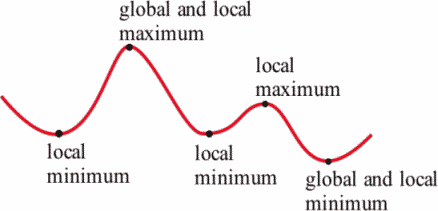
\includegraphics[width=0.4\textwidth]{img/chap3/image056.png}
    \caption{Local and global extrema}
    \label{fig:3-4-extrema}
\end{figure}

If $h(x)$ is the height of the earth above sea level at the location $x$, then the global maximum of $h(x)$ is the elevation at the summit of Mt.\ Everest, $29{,}031.7$ feet. The local maximum of $h(x)$ for the United States is the elevation at the summit of Denali (formerly Mt.\ McKinley), $20{,}310$ feet. The local minimum of $h(x)$ for the United States is the lowest point of Death Valley, $-282$ feet.

\begin{example}
Table \ref{tab:3-4-enrollment} shows the annual calculus enrollments at a large university. 
    \begin{enumerate}[label=(\alph*)]
    \item Which years had local maximum or minimum calculus enrollments? 
    \item What were the global maximum and minimum enrollments in calculus?
    \end{enumerate}
\begin{table}[ht!]
\begin{centering}
\begin{tabular}{*{12}{r}}
\toprule
{\bf Year:}         & 2000	& 2001	& 2002	& 2003	& 2004	& 2005	& 2006	& 2007	& 2008	& 2009	& 2010\tabularnewline
\midrule
{\bf Enrollment:}   & 1257	& 1324	& 1378	& 1336	& 1389	& 1450	& 1523	& 1582	& 1567	& 1545	& 1571\tabularnewline
\bottomrule
\end{tabular}
\caption{Calculus enrollments at a large university from 2000-2010}
\label{tab:3-4-enrollment}
\end{centering}
\end{table}
			
\begin{solution} 
    \begin{enumerate}[label=(\alph*)]
    \item There were local maxima in 2002 and 2007 since $1378> 1324, 1336$ and $1582> 1523, 1567$. There were local minima in 2003 and 2009 since $1336<1378, 1389$ and $1545< 1567, 1571$.
    \item The global maximum was 1582 students in 2007. The global minimum was 1257 students in 2000. 
    \end{enumerate}
    Note: We choose not to think of the 1257 students in 2000 or the 1571 students in 2010 as local extrema, but some books would include the endpoints. We may have global extrema at an endpoint of the domain.
\end{solution}
\end{example}

\subsection{Finding Extrema of a Function}
What must the tangent line look like at a local maximum or minimum? Look at the graph in Figure \ref{fig:3-4-find}. At all the extreme points, either the tangent line is horizontal, like at the points $a$, $c$, $e$, and $g$, or the tangent line doesn't exist, like at the cusp at the point $f$. It follows that at these extrema, either the derivative of the function is $0$ or is undefined.
\begin{figure}[!ht]
  \centering
    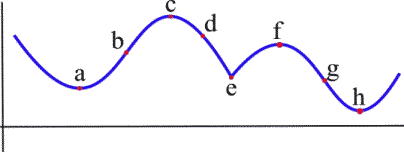
\includegraphics[width=0.4\textwidth]{img/chap3/image047.png}
    \caption{Local and global extrema}
    \label{fig:3-4-find}
\end{figure}
This gives us the method to find extreme values of a function.

\begin{definition}
    \begin{itemize}[label={}]
    \item A {\bf critical number}\index{Critical number} of a function $f(x)$ is a value $x=a$ in the domain of $f(x)$ where either $f'(a)=0$ or $f'(a)$ is undefined.
    \item A {\bf critical point}\index{Critical point}\index{Point!critical} of a function $f(x)$ is a point {(a, f(a))} where $a$ is a critical number of $f(x)$.
    \end{itemize}
\end{definition}

\begin{theorem}
A local maximum or local minimum of a function can only occur at a critical point of the function.
\end{theorem}

\begin{example}
\label{ex:3-4-critical}
Find the critical points of $f(x)=x^3-6x^2+9x+2$.

\begin{solution} A critical number of $f(x)$ can occur only where $f'(x)=0$ or where $f'(x)$ does not exist.

$$f'(x)=3x^2-12x+9=3(x^2-4x+3)=3(x-1)(x-3)$$
So $f'(x)=0$ at $x=1$ and $x=3$ (and no other values of $x$). There are no places where $f'(x)$ is undefined. Therefore, the critical numbers of $f(x)$ are $x=1$ and $x=3$, so the critical points of $f(x)$ are $(1, f(1)) = (1, 6)$ and $(3, f(3)) = (3, 2)$.
\end{solution}
\end{example}

We haven't discussed yet how to tell whether either of these points is actually a local extremum of $f(x)$, and if so, which kind of extremem it is. We can be certain, though, that no other point is a local extremum. The graph of $f(x)=x^3-6x^2+9x+2$ in Figure \ref{fig:3-4-fx} shows that the point $f(1)=6$ is a local maximum and $f(3)=2$ is a local minimum of $f(x)$. This function does not have a global maximum or minimum.

\begin{figure}[!ht]
  \centering
    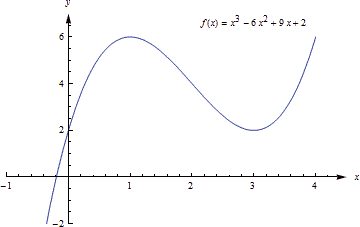
\includegraphics[width=0.4\textwidth]{img/chap3/image058.png}
    \caption{$f(x)=x^3-6x^2+9x+2$}
    \label{fig:3-4-fx}
\end{figure}

\begin{example}
Find all local extrema of $f(x)=x^3$.

\begin{solution} $f(x)=x^3$ is differentiable for all $x$, and $f'(x)=3x^2$. The only place where $f'(x)=0$ is at $x=0$, so the only candidate is the critical point $(0,0)$. Notice that if $x>0$, then $f(x)=x^3>0=f(0)$, so $f(0)$ is not a local maximum. Similarly, if $x<0$ then $f(x)=x^3<0=f(0)$ so $f(0)$ is not a local minimum.

Therefore, $f(x)=x^3$ does not have a local extremum.

Figure \ref{fig:3-4-cube} plots this function. We see, graphically, that this function does not have an extremum. The critical point is a {\bf saddle point}\index{Saddle point}\index{Point!saddle}.
\begin{figure}[!ht]
  \centering
    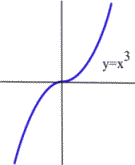
\includegraphics[width=0.2\textwidth]{img/chap3/image059.png}
    \caption{$f(x)=x^3$}
    \label{fig:3-4-cube}
\end{figure}
\end{solution}
\end{example}

Remember this example! It is not enough to find the critical points -- we can only say that $f(x)$ {\em might} have a local extremum at any critical point.

\subsection{First and Second Derivative Tests}

\paragraph*{Is that critical point a Maximum, Minimum, or Neither?}
Once we have found the critical points of $f(x)$, we still have the problem of determining whether these points are maxima, minima, or neither.

All of the graphs in Figure \ref{fig:3-4-6examples} have a critical point of $(2, 3)$. It is clear from the graphs that the point $(2,3)$ is a local maximum in (a) and (d), $(2,3)$ is a local minimum in (b) and (e), and $(2,3)$ is not a local extremum in (c) and (f).

\begin{figure}[!ht]
  \centering
    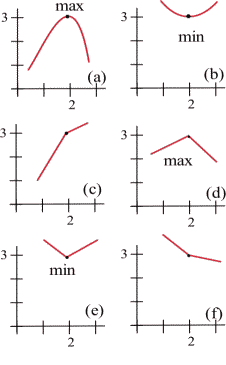
\includegraphics[width=0.4\textwidth]{img/chap3/image060.png}
    \caption{Six examples}
    \label{fig:3-4-6examples}
\end{figure}

The critical numbers only give the possible locations of extrema, and some critical numbers are not the locations of extrema. The critical numbers are the candidates for the locations of maxima and minima.

\paragraph*{$f'(x)$ and Extrema of $f(x)$}
Four possible shapes of graphs are shown in Figure \ref{fig:3-4-1derivtest}. In each graph, the point marked by an arrow is a critical point, where $f'(x)=0$. What happens to the derivative near the critical point?

\begin{figure}[!ht]
  \centering
    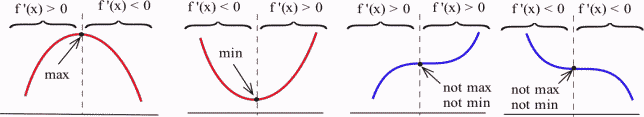
\includegraphics[width=0.7\textwidth]{img/chap3/image061.png}
    \caption{Six examples}
    \label{fig:3-4-1derivtest}
\end{figure}

At a local maximum, such as in the graph on the left, the function increases on the left of the local maximum, then decreases on the right. The derivative is first positive, then negative at a local maximum. At a local minimum, the function decreases to the left and increases to the right, so the derivative is first negative, then positive. When there isn't a local extreme, the function continues to increase (or decrease) right past the critical point -- the derivative doesn't change sign. This is the argument and picture behind the first test we have to identify the kind of point a critical point is.

\begin{theorem}[The First Derivative Test for Extrema\index{First Derivative Test}]
Suppose that $f(x)$ is a function defined in a neighborhood around a critical value\index{Critical value} $x=c$, so that $(c, f(c))$ is a critical point\index{Critical point}\index{Point!critical}. Suppose we examine the sign of $f'(x)$ to the left and to the right of $x=c$. 
    \begin{itemize}
    \item If $f'(x)$ changes from positive to negative at $x=c$, then $f(c)$ is a {\bf local maximum}\index{Local maximum}\index{Maximum!local}\index{Relative maximum}\index{Maximum!relative} of $f(x)$.
    \item If $f'(x)$ changes from negative to positive at $x=c$, then $f(c)$ is a {\bf local minimum}\index{Local minimum}\index{Minimum!local}\index{Relative minimum}\index{Minimum!relative} of $f(x)$.
    \item If $f'(x)$ does not change sign at $x=c$, then $f(c)$ is neither a local maximum nor a local minimum.
    \end{itemize}
\end{theorem}
\begin{example}
Find the critical points of $f(x)=x^3-6x^2+9x+2$ and classify them as local maximum, local minimum, or neither.

\begin{solution} We already found the critical points of $f(x)$ in Example \ref{ex:3-4-critical}: $(1, 6)$ and $(3, 2)$.

Now we can use the first derivative test to classify each. We have $f'(x)=3x^2-12x+9=3(x^2-4x+3)=3(x-1)(x-3)$. The factored form is easiest to work with here, so let's use that.

At the point $(1, 6)$, we could choose a number slightly less than 1 to plug into $f'(x)$ -- perhaps use $x=0$ or $x=0.9$. Then we examine its sign. We don't care about the numerical value. We just need to know if $f'(x)<0$ or $f'(x)>0$. Since $f'(x)$ is factored, we don't have to actually plug anything in.
    \begin{itemize}
    \item If $x<1$, then $x-1<0$ and $x-3<0$, so $f'(x)=3(x-1)(x-3) = (+)(-)(-) > 0$; a positive times a negative times a negative is positive.
    \item If $1<x<3$, that is, between the critical values, then we can do the same thing. We evaluate $f'(x)$ at a number between 1 and 3, perhaps $x=2$. Or we can make a quick sign argument like what we did above: for $x$ a little more than 1, $f'(x)=3(x-1)(x-3)=(+)(+)(-)<0$. 
    \item If $x>3$, then $x-1>0$ and $x-3>0$, so $f'(x)=3(x-1)(x-3) = (+)(+)(+) > 0$;
    \end{itemize}
So $f'(x)$ changes signs from positive to negative around $x=1$, which means there is a local maximum at the point $(1, 6)$; 6 is the local maximum. Also, $f'(x)$ changes signs from negative to positive around $x=3$, which means there is a local minimum at the point $(3, 2)$; 2 is the local minimum. 

As another approach, we could draw a number line, and mark the critical numbers.
\begin{figure}[!ht]
  \centering
    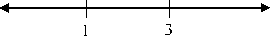
\includegraphics[width=0.5\textwidth]{img/chap3/image109.png}
    %\caption{Number line with critical values of $f(x)$.}
    %\label{fig:3-4-1derivtest}
\end{figure}
We already know that $f'(1)=f'(3)=0$. On each interval between these values, the derivative will stay the same sign. To determine the sign, we could pick a test value in each interval, and evaluate the derivative at those points (or use the sign approach used above).
\begin{figure}[!ht]
  \centering
    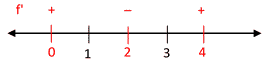
\includegraphics[width=0.5\textwidth]{img/chap3/image110.png}
    %\caption{Six examples}
    %\label{fig:3-4-1derivtest}
\end{figure}
\end{solution}
\end{example}

\paragraph*{$f''(x)$ and Extrema of $f(x)$}
The concavity\index{Concavity} of a function can also help us determine whether a critical point is a maximum, minimum, or neither. For example, if a point is at the bottom of a concave up function, then the point is a minimum.

\begin{figure}[!ht]
  \centering
    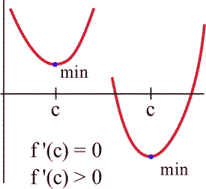
\includegraphics[width=0.4\textwidth]{img/chap3/image062.png}
    %\caption{Six examples}
    %\label{fig:3-4-1derivtest}
\end{figure}

\begin{theorem}[The Second Derivative Test for Extrema\index{Second Derivative Test}]
Suppose $(c, f(c))$ is a critical point\index{Critical point}\index{Point!critical} of $f(x)$, $f'(c)=0$, and $f''(c)$ exists.
    \begin{itemize}
    \item If $f''(c)<0$, then $y=f(x)$ is {\bf concave down}\index{Concave down} and $f(c)$ is a {\bf local maximum}\index{Local maximum}\index{Maximum!local} of $f(x)$.
    \item If $f''(c)>0$, then $y=f(x)$ is {\bf concave up}\index{Concave up} and $f(c)$ is a {\bf local minimum}\index{Local minimum}\index{Minimum!local} of $f(x)$.
    \item If $f''(c)=0$ then the test is {\bf inconclusive}; $f(x)$ may have a local maximum, a minimum, or neither at $x=c$.
    \end{itemize}
\end{theorem}
The cartoon faces in Figure \ref{fig:3-4-2derivtest} can help you remember the Second Derivative Test.

\begin{figure}[!ht]
  \centering
    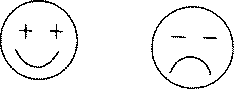
\includegraphics[width=0.4\textwidth]{img/chap3/image063.png}
    \caption{Visualizing the Second Derivative Test}
    \label{fig:3-4-2derivtest}
\end{figure}

\begin{example}
$f(x)=2x^3-15x^2+24x-7$ has critical numbers $x= 1$ and 4. Use the Second Derivative Test for extrema to determine whether $f(1)$ and $f(4)$ are maxima, minima, or neither.

\begin{solution} We need to find the second derivative:
\begin{align*}
		f(x) &= 2x^3 - 15x^2 + 24x - 7\\
		f'(x) &= 6x^2 - 30x + 24\\
		f''(x) &= 12x - 30
	\end{align*}
Then we just need to evaluate $f''(x)$ at each critical number.
    \begin{itemize}[label={}]
    \item $x=1$: $f''(1)=12(1)-30<0$, so $f(1)=4$ is a local maximum of $f(x)$.
    \item $x=4$: $f''(4)=12(4)-30>0$, so $f(4)=-23$ is a local minimum of $f(x)$.
    \end{itemize}
\end{solution}
\end{example}

Many students like the Second Derivative Test. The Second Derivative Test is often easier to use than the First Derivative Test. You only have to find the sign of one number for each critical number rather than two. And if your function is a polynomial, its second derivative will probably be a simpler function than the derivative.

However, if you needed a product rule, quotient rule, or chain rule to find the first derivative, finding the second derivative can be a lot of work. Also, even if the second derivative is easy, the Second Derivative Test doesn't always give an answer. The First Derivative Test will always give you an answer.

Use whichever test you want to. But remember -- you have to do some test to be sure that your critical point actually is a local maximum or minimum.

\subsection{Global Maxima and Minima\index{Global extremum}\index{Extremum!global}\index{Global maximum}\index{Global minimum}\index{Maximum!global}\index{Minimum!global}}
In applications, we often want to find the global extrema; knowing that a critical point is a local extreme is not enough.

For example, if we want to make the greatest profit. we want to make the absolutely greatest profit of all. How do we find global maximum and minimum of a function?

There are just a few additional things to think about.

\paragraph*{Endpoint Extrema} 
The local extrema of a function occur at critical points -- these are points in the function that we can find by thinking about the shape (and using the derivative to help us). But if we're looking at a function on a closed interval, the endpoints could be extrema. These endpoint extrema are not related to the shape of the function; they have to do with the interval, the window through which we're viewing the function.

\begin{figure}[!ht]
  \centering
    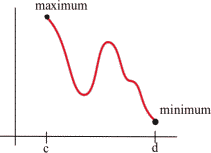
\includegraphics[width=0.4\textwidth]{img/chap3/image064.png}
    \caption{Global Extrema at Domain Endpoints}
    \label{fig:3-4-globalextrema}
\end{figure}
In Figure \ref{fig:3-4-globalextrema}, it appears that there are three critical points -- one local minimum, one local maximum, and one saddle point. But the global maximum, the highest point of all, is at the left endpoint. The global minimum, the lowest point of all, is at the right endpoint.

How do we decide if an endpoint is a global maximum or minimum? It's easier than you expected -- simply plug in the endpoints, along with all the critical numbers, and compare $y$-values.

\begin{theorem}
If $f(x)$ is a continuous function on a closed domain: $a\le x\le b$, then $f(x)$ has a {\bf global maximum} and a {\bf global minimum}. Global extrema will occur at:
    \begin{itemize}
    \item $x=a$ (the left endpoint of the domain),
    \item $x=b$ (the right endpoint of the domain), or
    \item a critical value of $f(x)$.
    \end{itemize}
\end{theorem}

\begin{example}
Find the global maximum and minimum of $f(x)=x^3-3x^2-9x+5$ for $-2\le x\le 6$.

\begin{solution} $f'(x)=3x^2-6x-9=3(x+1)(x-3)$. We need to find critical points and we need to check the endpoints, $x=-2$ and $x=6$.

$f'(x)=3(x+1)(x-3)=0$ when $x=-1$ and $x=3$.

Now we simply compare the values of $f(x)$ at these four values of $x$.

\begin{center}
\begin{tabular}{rr}
\toprule
$x$     & $f(x)$ \\
\midrule
$-2$    &    3 \\
$-1$    &	10	\\
3       &	$-22$ \\
6       &	59 \\
\bottomrule
\end{tabular}
\end{center}

The global minimum of $f(x)$ on $[-2,6]$ is $-22$, when $x=3$, and the global maximum of $f(x)$ on $[-2,6]$ is 59, when $x=6$.
\end{solution}
\end{example}

\paragraph*{If there's only one critical point}
If the function has only one critical point and it's a local maximum (or minimum), then it must be the global maximum (or minimum). To see this, think about the geometry. Look at the graph on the left in Figure \ref{fig:3-4-65} -- there is a local maximum, and the graph goes down on either side of the critical point. Suppose there was some other point that was higher -- then the graph would have to turn around. But that turning point would have shown up as another critical point. If there's only one critical point, then the graph can never turn back around.

\begin{figure}[!ht]
  \centering
    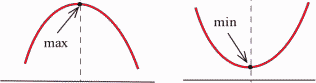
\includegraphics[width=0.4\textwidth]{img/chap3/image065.png}
    \caption{Global Extrema at Critical Points}
    \label{fig:3-4-65}
\end{figure}
\paragraph*{When in doubt, graph it and look.}
If you are trying to find a global maximum or minimum on an open interval (or the whole real line), and there is more than one critical point, then you need to look at the graph to decide whether there is a global maximum or minimum. Be sure that all your critical points show in your graph, and that you graph beyond them -- that will tell you what you want to know.

\begin{example}
Find the global maximum and minimum of $f(x)=x^3-6x^2+9x+2$.

\begin{solution} We have previously found that $f(1) = 6$ is a local maximum and $f(3)= 2$ is a local minimum. This is not a closed interval, and there are two critical points, so we must turn to the graph of the function to find global extrema.

The graph of $f(x)$ shows that points to the left of $x=4$ have $y$-values greater than 6, so $f(1)= 6$ is not a global maximum. Likewise, if $x$ is negative, then $y$ is less than 2, so $2$ is not a global minimum. There are no endpoints, so we've exhausted all the possibilities. This function does not have a global maximum or minimum.

\begin{figure}[!ht]
  \centering
    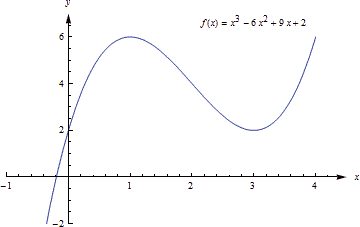
\includegraphics[width=0.4\textwidth]{img/chap3/image058.png}
    %\caption{Global Extrema at Critical Points}
    %\label{fig:3-4-65}
\end{figure}
\end{solution}
\end{example}

\begin{theorem}[Finding Global Extrema]
The only places where a function can have a global extreme are critical points or endpoints of the domain.
    \begin{itemize}
    \item If the function has only one critical point, and it's a local extremum, then it is also a global extremum.
    \item If the domain has endpoints, find the global extrema by comparing $y$-values at all the critical points and at the endpoints.
    \item When in doubt, graph the function to be sure. (However, unless the problem explicitly tells you otherwise, it is not enough to just use the graph to get your answer.)
    \end{itemize}
\end{theorem}
